\documentclass[11pt,a4paper]{article}
\usepackage[margin=18mm,headheight=15pt]{geometry}
\usepackage[T1]{fontenc}
\usepackage{lmodern,amsmath,amssymb,booktabs,array,enumitem,fancyhdr,xcolor}
\usepackage[american]{circuitikz}
\usepackage[hidelinks]{hyperref}
\definecolor{ink}{HTML}{17324D}
\pagestyle{fancy}\fancyhf{}\lhead{\small Electronic Circuits I}\rhead{\small Worked solutions | 30 marks}\cfoot{\small\thepage}
\setlength{\parindent}{0pt}\setlength{\parskip}{6pt}
\setlist[enumerate]{leftmargin=*,itemsep=7pt,topsep=4pt}
\newcommand{\q}[2]{\par\vspace{3pt}{\large\bfseries\color{ink}#1}\hfill\textbf{[#2 marks]}\par\hrule\vspace{7pt}}
\newcommand{\m}[1]{\hfill\textbf{[#1]}}
\newcommand{\kohm}{\,\mathrm{k}\Omega}
\newcommand{\uF}{\,\mu\mathrm{F}}
\begin{document}

{\Huge\bfseries\color{ink}Worked solutions}\par
{\large Electronic Circuits I --- Practice midterm}\par
\textit{Attempt the paper before reading this file. The marking guide is proposed for practice; it is not the lecturer's official rubric. Equivalent valid methods earn credit.}
\q{Question 1}{5}
\textbf{(a) Three-op-amp realization [3].} Use an inverting differentiator, an inverting integrator, and an inverting summer:
\[
u_1=-R_dC_d\frac{dv_1}{dt},\qquad
u_2=-\frac{1}{R_iC_i}\int_0^t v_2(\tau)d\tau,
\]
\[
v_o=-\frac{R_f}{R_a}u_1-\frac{R_f}{R_b}u_2-\frac{R_f}{R_c}v_3.
\]
Choose $R_d=10\kohm$, $C_d=100$ nF, $R_i=100\kohm$, $C_i=100$ nF, $R_f=R_a=R_b=20\kohm$, and $R_c=10\kohm$. Both processing stages invert; the summer inverts again, producing positive derivative and integral terms and the required negative $v_3$ term.
\begin{center}\begin{circuitikz}[scale=.72,transform shape]
\draw (3,0) node[op amp](a){};
\draw (-.5,.49) node[left]{$v_1$} to[C,l={$C_d$}] (a.-);
\draw (a.+) -- ++(0,-.5) node[ground]{};
\draw (1.6,.49) to[short,*-] (1.6,2) to[R,l={$R_d$}] (4.4,2) -- (4.4,0);
\draw (a.out) to[short,-o] (4.7,0) node[right]{$u_1$};
\draw (10,0) node[op amp](b){};
\draw (6.5,.49) node[left]{$v_2$} to[R,l={$R_i$}] (b.-);
\draw (b.+) -- ++(0,-.5) node[ground]{};
\draw (8.6,.49) to[short,*-] (8.6,2) to[C,l={$C_i$}] (11.4,2) -- (11.4,0);
\draw (b.out) to[short,-o] (11.7,0) node[right]{$u_2$};
\end{circuitikz}
\begin{circuitikz}[scale=.78,transform shape]
\draw (5,0) node[op amp](s){};
\draw (0,2) node[left]{$u_1$} to[R,l={$R_a$}] (2.5,2) -- (2.5,.49) -- (s.-);
\draw (0,.49) node[left]{$u_2$} to[R,l={$R_b$}] (2.5,.49);
\draw (0,-1) node[left]{$v_3$} to[R,l={$R_c$}] (2.5,-1) -- (2.5,.49);
\draw (s.+) -- ++(0,-.8) node[ground]{};
\draw (3.5,.49) to[short,*-] (3.5,2.5) to[R,l={$R_f$}] (6.4,2.5) -- (6.4,0);
\draw (s.out) to[short,-o] (7,0) node[right]{$v_o$};
\end{circuitikz}\end{center}
\textbf{Marking:} correct topology and signs 1.5; coefficient relations 0.75; consistent values 0.75. All noninverting inputs are grounded. The ideal differentiator is the course model; practical bandwidth limiting is outside this question.

\textbf{(b) Finite gain [1].} Let $\alpha=R_g/(R_g+R_f)=0.1$. Then
\[
v_o=A_0(v_i-\alpha v_o),\quad A_{CL}=\frac{A_0}{1+A_0\alpha}
=\frac{1000}{101}=9.90099.
\]
The ideal gain is 10, so the reduction is $(10-9.90099)\times100/10=0.9901\%$. Award 0.5 for derivation and 0.5 for numerical result.

\textbf{(c) Log amplifier [1].} For positive input, the feedback transistor carries $I\simeq v_{\rm in}/R>0$ and gives a logarithmic relation. Negative input would require reverse feedback current, invalidating this forward-conduction model and the real logarithm. The circuit loses its intended logarithmic feedback behavior; the output may run toward a rail. A bipolar-input log circuit needs a different topology.
\newpage
\q{Question 2}{7}
\textbf{(a) R--2R derivation [2].} For code 0010, only $b_1$ is high. With $b_0=0$, the termination and the $b_0$ branch give $2R\parallel2R=R$. The path from the $b_1$ junction toward ground is thus $R+R=2R$. Its Thevenin equivalent is
\[
V_{\rm th,1}=V_{\rm ref}/2,\qquad R_{\rm th,1}=R.
\]
Moving one section right, the zero-valued $b_2$ branch produces
\[
V_{\rm th,2}=V_{\rm ref}/4,\qquad R_{\rm th,2}=R.
\]
The final series $R$ feeds the virtual ground at the MSB junction:
\[
I_{0010}=\frac{V_{\rm ref}/4}{R+R}=\frac{V_{\rm ref}}{8R},
\qquad v_o(0010)=-\frac{R_f}{R}\frac{V_{\rm ref}}8.
\]
By superposition,
\[
\boxed{v_o=-\frac{R_f}{R}V_{\rm ref}
\left(\frac{b_3}{2}+\frac{b_2}{4}+\frac{b_1}{8}+\frac{b_0}{16}\right)
=-\frac{R_fV_{\rm ref}}{16R}N.}
\]
Here $N=8b_3+4b_2+2b_1+b_0$. Award 1.5 for the single-bit derivation and 0.5 for the general expression.

\textbf{(b) Design [2].} The MSB sees its $2R$ resistor terminating at virtual ground, so $2R=20\kohm$ and $R=R_f=10\kohm$. At $N=15$,
\[
-3.75=-V_{\rm ref}\frac{15}{16}\quad\Rightarrow\quad V_{\rm ref}=4\,\mathrm V.
\]
\begin{center}\begin{tabular}{ccccc}\toprule
$R$ & $2R$ & $R_f$ & Logic 0 & Logic 1\\\midrule
$10\kohm$ & $20\kohm$ & $10\kohm$ & 0 V & 4 V\\\bottomrule\end{tabular}\end{center}
The signed step is $\Delta v_o=-4/16=-0.25$ V per code. Code $1011$ has $N=11$, giving $v_o=-2.75$ V. Award 0.5 each for resistance choice, reference, step, and code output.

\textbf{(c) ADC sequence [2].}
\begin{center}\begin{tabular}{c*{6}{c}}\toprule
Sample &1&2&3&4&5&6\\
$v_{\rm in}$ (V)&0.4&1.2&2.6&3.4&2.2&0.8\\
$C_3C_2C_1$&000&001&011&111&011&000\\
$D_1D_0$&00&01&10&11&10&00\\\bottomrule\end{tabular}\end{center}
\begin{center}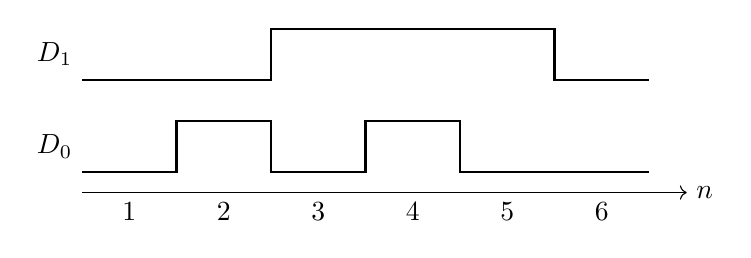
\begin{tikzpicture}[x=1.2cm,y=.65cm]
\draw[->] (0,-.2)--(6.4,-.2) node[right]{$n$};
\foreach \x in {1,...,6}{\node[below] at (\x-.5,-.2){\x};}
\node[left] at (0,2.5){$D_1$};\node[left] at (0,.7){$D_0$};
\draw[thick] (0,2)--(2,2)--(2,3)--(5,3)--(5,2)--(6,2);
\draw[thick] (0,.2)--(1,.2)--(1,1.2)--(2,1.2)--(2,.2)--(3,.2)--(3,1.2)--(4,1.2)--(4,.2)--(6,.2);
\end{tikzpicture}\end{center}
Award 1 for codes and comparator states, 1 for both digital waveforms.

\textbf{(d) Comparator interpretation [1].} Step size $=4/4=1$ V; a 3-bit flash ADC requires $2^3-1=7$ comparators. These op-amps operate open-loop as comparators, with no linear negative-feedback constraint. Thus their inputs generally differ and their outputs select a logic level. Award 0.25, 0.25, and 0.5 respectively.
\newpage
\q{Question 3}{3}
\textbf{(a) [1].} A 7812 provides nominally $+12$ V. At the onset of external-transistor conduction,
\[
R_{\rm ext}=\frac{0.70}{0.40}=1.75\,\Omega.
\]
\textbf{(b) [1].} $I_L=12/12=1$ A. Under the stated current-sharing model, the external transistor supplies $1-0.40=0.60$ A, and dissipates
\[
P_Q=(18-12)(0.60)=3.60\,\mathrm W.
\]
This is calculated electrical dissipation, not a complete heat-sink specification.

\textbf{(c) [1].} The external transistor bypasses the IC's internal limiting path. Add a sense resistor in series with the total output current and a sensing transistor that, at the threshold, reduces pass-device drive through the control/feedback path. The sense resistor is
\[
R_s=\frac{0.70}{1.50}=0.467\,\Omega.
\]
Award 0.5 for the protection mechanism and 0.5 for the value. A correct equivalent circuit proposal is acceptable. The sensing arrangement must act on total current, rather than only the IC branch.
\q{Question 4}{4}
\textbf{(a) Standard astable [2].} $V_L=V_{CC}/3=3$ V and $V_H=2V_{CC}/3=6$ V. The capacitor charges through $R_A+R_B$ and discharges through $R_B$:
\[
t_H=(\ln2)(R_A+R_B)C,\quad t_L=(\ln2)R_BC.
\]
For $T=1$ ms and $D=0.75$, $t_H=0.75$ ms and $t_L=0.25$ ms:
\[
R_B=\frac{0.25\,\mathrm{ms}}{(\ln2)(100\,\mathrm{nF})}=3.607\kohm,
\]
\[
R_A=\frac{0.75\,\mathrm{ms}}{(\ln2)(100\,\mathrm{nF})}-R_B=7.213\kohm.
\]
Award 0.5 for thresholds, 0.5 for equations, and 1 for resistor values.

\textbf{(b) Modified astable [2].} Place a diode across $R_B$, with \textbf{anode at pin 7 and cathode at the timing-capacitor node (pins 2/6)}. It bypasses $R_B$ during charging and is reverse-biased during discharge.
\begin{center}\begin{circuitikz}[scale=.8,transform shape]
\draw (0,4) node[above]{$V_{CC}$} to[R,l={$R_A$}] (0,2.3) to[R,l={$R_B$}] (0,.3) to[C,l={$C$}] (0,-1.2) node[ground]{};
\draw (0,2.3) to[short,*-] (2,2.3) to[D,l={$D$}] (2,.3) to[short,-*] (0,.3);
\draw (0,2.3) -- (-1.5,2.3) node[left]{pin 7};
\draw (0,.3) -- (-1.5,.3) node[left]{pins 2/6};
\end{circuitikz}\end{center}
Now $t_H=(\ln2)R_AC$ and $t_L=(\ln2)R_BC$, hence
\[
R_A=\frac{0.40\,\mathrm{ms}}{(\ln2)C}=5.771\kohm,\qquad
R_B=\frac{0.60\,\mathrm{ms}}{(\ln2)C}=8.656\kohm.
\]
Without the diode, $D=(R_A+R_B)/(R_A+2R_B)>1/2$ for positive resistors. Award 0.75 for modification/orientation, 1 for values, and 0.25 for the limitation. Values computed using 0.693 or 1.44 are acceptable within rounding.
\newpage
\q{Question 5. DC and bypassed CE stage}{6 of 11}
\textbf{(a) Physical operation [1].} The forward-biased emitter junction injects electrons into the thin p-type base. Most diffuse across the neutral base without recombining; the reverse-biased collector junction's electric field sweeps them into the collector. Transport through the neutral base is predominantly diffusion. The two junctions share a thin base, so two independent back-to-back diodes do not model this action.

\textbf{(b) Bias [3].} For DC, all capacitors are open, isolating the source and load:
\[
V_{\rm th}=8\frac{20}{60+20}=2\,\mathrm V,\qquad
R_{\rm th}=60\kohm\parallel20\kohm=15\kohm.
\]
Using $I_E=(\beta+1)I_B$,
\[
I_B=\frac{V_{\rm th}-V_{BE}}{R_{\rm th}+(\beta+1)R_E}
=\frac{1.3}{116\kohm}=11.207\,\mu\mathrm A.
\]
\[
I_C=1.12069\,\mathrm{mA},\quad I_E=1.13190\,\mathrm{mA},\quad
V_E=1.13190\,\mathrm V,\quad V_B=1.83190\,\mathrm V.
\]
\[
V_C=8-I_CR_C=4.63793\,\mathrm V,\qquad
\boxed{V_{CE}=3.50603\,\mathrm V.}
\]
Since $V_B-V_E=0.70$ V and $V_C>V_B$, the BE junction is forward biased and the BC junction is reverse biased. The active-region assumption is consistent. Award 0.5 for the Thevenin pair, 1 for currents, 1 for voltages, and 0.5 for the region check.

\textbf{(c) Midband model and parameters [2].} $C_E$ grounds the emitter for AC, and the DC supply is AC ground. The bias resistors remain in parallel at the input.
\begin{center}\begin{circuitikz}[scale=.85,transform shape]
\draw (0,3) node[above]{$v_i=v_\pi$} to[R,l_={$R_1\parallel R_2$}] (0,0) node[ground]{};
\draw (0,3) to[short,*-] (2.3,3) to[R,l={$r_\pi$}] (2.3,0) node[ground]{};
\draw (5,3) to[cisource,l_={$g_mv_\pi$}] (5,0) node[ground]{};
\draw (5,3) -- (7,3) node[above]{$v_o$} to[R,l={$R_C$}] (7,0) node[ground]{};
\draw (7,3) to[short,*-] (9.3,3) to[R,l={$R_L$}] (9.3,0) node[ground]{};
\end{circuitikz}\par\small Controlled-source current is from collector to emitter (downward).\end{center}
\[
g_m=\frac{I_C}{V_T}=44.8276\,\mathrm{mS},\qquad
r_\pi=\frac{\beta}{g_m}=2.23077\kohm.
\]
\[
A_v=-g_m(R_C\parallel R_L)=-0.0448276(2000)=-89.655,
\]
\[
R_{\rm in}=R_1\parallel R_2\parallel r_\pi=1.94196\kohm,
\qquad R_{\rm out}=R_C=3\kohm.
\]
Award 0.5 for the model, 0.5 for $g_m,r_\pi$, 0.5 for gain and 0.5 for both impedances. If a finite Early voltage were specified, $r_o$ would be included; it is infinite here by assumption.
\newpage
\q{Question 5. Degeneration, follower and CB}{5 of 11}
\textbf{(d) Remove the bypass capacitor [2].} Write $v_i=i_b r_\pi+i_eR_E$ with $i_e=(\beta+1)i_b$. The collector signal is $v_o=-\beta i_b(R_C\parallel R_L)$. Therefore,
\[
\boxed{A_v=-\frac{\beta(R_C\parallel R_L)}{r_\pi+(\beta+1)R_E}}
=-\frac{100(2000)}{2230.77+101(1000)}=-1.93741.
\]
\[
\boxed{R_{\rm in}=R_1\parallel R_2\parallel[r_\pi+(\beta+1)R_E]}
=13.0969\kohm.
\]
The DC operating point is unchanged because the bypass capacitor was already open in DC. Degeneration decreases gain magnitude and increases input resistance. Award 1 for gain derivation/result, 0.75 for input resistance, and 0.25 for the DC conclusion.

\textbf{(e) Emitter follower [2].} Here $r_\pi=100/0.040=2.5\kohm$ and the loaded emitter resistance is $R_E'=1\kohm\parallel1\kohm=500\,\Omega$. Since the ideal base bias current source has infinite small-signal impedance,
\[
R_{\rm in,base}=r_\pi+(\beta+1)R_E'=2500+101(500)=53\kohm,
\]
\[
\boxed{\frac{v_e}{v_b}=\frac{(\beta+1)R_E'}{r_\pi+(\beta+1)R_E'}
=\frac{50500}{53000}=0.95283.}
\]
This is the requested \emph{base-to-emitter} gain. The source resistance is not included in that ratio. If one instead wanted source-to-output gain, it would be $0.95283\times53/(53+3)=0.90179$.

For output resistance, remove $R_L$, set the signal source to zero, and retain $R_s$ from base to ground:
\[
\boxed{R_{\rm out}=R_E\parallel\frac{r_\pi+R_s}{\beta+1}}
=1000\parallel\frac{2500+3000}{101}=51.643\,\Omega.
\]
Award 0.5 for input resistance, 0.5 for gain, and 1 for output resistance including the source resistance and correct load removal.

\textbf{(f) Common-base stage [1].} $g_m=1\,\mathrm{mA}/25\,\mathrm{mV}=40$ mS and $r_\pi=2.5\kohm$. The base is AC ground, so $v_\pi=-v_e$. KCL at the collector gives $v_c=+g_mR_C'v_e$:
\[
\boxed{A_v=+0.04(2000)=+80,}\qquad
\boxed{R_{\rm in,e}=\frac{1}{g_m+1/r_\pi}=\frac{r_\pi}{\beta+1}=24.7525\,\Omega.}
\]
The large-$\beta$ approximation is $1/g_m=25\,\Omega$. Award 0.5 for each quantity; accept the approximation if stated.

\vfill
\textbf{Mark check:} $5+7+3+4+11=30$. Carry a consistent earlier numerical error forward without repeatedly penalizing it. Deduct separately for a new conceptual error (for example, neglecting the load in the gain or imposing a virtual short on a comparator).
\end{document}
